
\title{HOME AUTOMATION\\ \normalsize  FEASIBILITY REPORT}
\author{
        \\
        Department of Electronics And Communication\\
       Govt.Model Engineering College\\
       Thrikkakara\\
       \\
       \\\textbf{TEAM MEMBERS}\\
       \\20 - Deepak  J Puthukkaden\\
        31 - Giridhar A K\\
        32 - Govindh B\\
        53 - Rohit Sreekumar\\
        59 - Shine Ali\\
}
%\date{}

\documentclass[12pt,a4paper,oneside]{report}


\usepackage{amsfonts}

\usepackage[english]{babel}
\usepackage{textcomp}
\usepackage{graphicx}
\usepackage{setspace}
\usepackage{fancyhdr}
\usepackage{truncate}
\usepackage{nomencl} 
\usepackage{array}
\usepackage{caption}
\usepackage{subcaption}
\usepackage{subfig}
\usepackage[overload]{textcase}
\renewcommand{\nomname}{List of Abbreviations}
\makenomenclature



\usepackage{titlesec}
\titleformat{\chapter}[display]
  {\normalfont\Large\bfseries\centering}
 {\chaptertitlename\ \thechapter}{20pt}{\LARGE}
\titleformat{\section}{\large\bfseries}{\thesection}{1em}{}
\titleformat{\subsection}{\normalsize\bfseries}{\thesubsection}{1em}{}



\renewcommand{\chaptermark}[1]{\markboth{ \emph{#1}}{}}

\begin{document}
\maketitle
\thispagestyle{empty}

\pagenumbering{roman}



\begin{onehalfspacing}



\pagenumbering{arabic}

\tableofcontents

\chapter{INTRODUCTION}
{$\;\;\;\;$}
  
The proposed idea for our Mini porject for the Fifth Semester (2014-2015) is Home Automation based on Raspberry Pi. Automation is a broad concept of engineering and home automation is but a small subsidiary of this vast idea. Recently, the idea of the Internet Of Things has gathered momentum and many interesting applications have surfaced making many of the daily chores simple and efficient. We intend to implement a small scale home automation project using the Raspberry Pi. The Raspberry Pi is a powerful credit card sized computer capable of running as a normal computer and also capable of running the functions of a microcontroller. 
\\Due to the hardware limitations(limited no of input and output pins) of the Raspberry Pi, we are forced to interface an additional microcontroller to control the various sensors involved in the automation.

\newpage
\section{Features of the project}
{$\;\;\;\;$}
The system comprises automation of some daily tasks in our home. They different functions of the system are:\\
\begin{itemize}
\item Adaptive Internal Lighting System
\item Temperature Monitoring
\item Automatic External Lighting
\item Automatic Water Pumping System
\item Password Enabled Door Lock system
\item Interactive Music Player
\item Data Logging and analysis 
\end{itemize}

\newpage



\subsection{Adaptive Internal Lighting System}
{$\;\;\;\;$}
The adaptive internal lighting system controls the amount of illumination in a room by controlling a light source, based on the amount of light present in the room. The sensor involved is a light dependant resistor(LDR) which varies it's resistance depending on the amount of light falling on it.The change in resistance will result in a change in the voltage drop accross the resistance(a varying analog signal).For demonstration purposes we intend to use an LED, the brightness of which is controlled using Pulse Width Modulation technique. 

\subsection{Temperature Monitoring}
{$\;\;\;\;$}
 This feature of our project collects the real time data related to the room temperature. This data can be used to control the air-conditioning or the speed of a fan. For demonstration, the temperature will be measured and stored in the Raspberry Pi.

\subsection{Automatic External Lighting}
{$\;\;\;\;$}
This feature of our project controls an external lighting system based on the amount of external light. When the light outside the home falls below a specific value, the light is turned on. It also makes use of a LDR

\subsection{Automatic Water Pumping System}
{$\;\;\;\;$}
 Through this system we intend to control the water pump based on the water level inside the water tank. This prevents the overflowing and wastage of water which is a pristine and scarce resource. The water level is determined by two sensors and the output is used by the Raspberry Pi to drive a relay that switches the water pumping system.

\newpage
\subsection{Password Enabled Door Lock system}
{$\;\;\;\;$}
This feature adds to the security of the smart home.A keypad is interfaced with the microcontroller which is then connected to a door lock system.The door lock gets unlocked when the correct password is entered.

\subsection{Interactive Music Player}
{$\;\;\;\;$}
This part of the project adds to the entertainment in the smart home. A simple music player is integrated with the Raspberry Pi which can be controlled using using small buttons for functions like play, paues etc.

\subsection{Holistic Data Logging}
{$\;\;\;\;$}
This feature comprises of the data logging and event tracking feature of our project. Data logging includes the temperature measurement and event logging. It can be used to analyse the working of the home.

\newpage
\section{Block diagram}
{$\;\;\;\;$}
\begin{figure}[h]
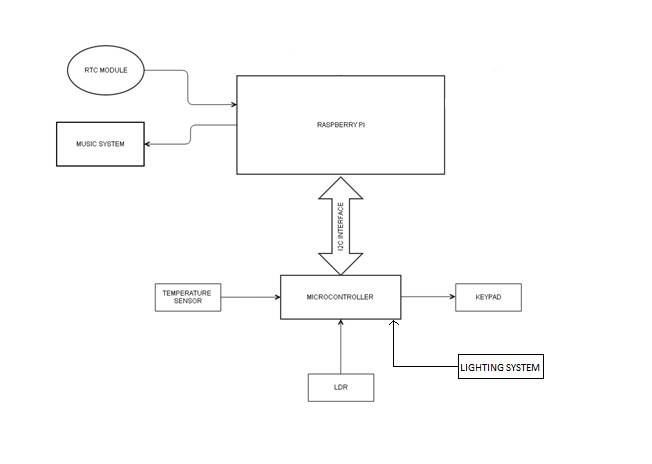
\includegraphics[width=15cm, height=6cm]{ABC.png}
\centering
\caption{Block Diagram}
\label{fig1}
\end{figure}



\section{Hardware Used}
{$\;\;\;\;$}
\subsection{Raspberry Pi}
The Raspberry Pi is a credit-card-sized single-board computer developed in the UK by the Raspberry Pi Foundation with the intention of promoting the teaching of basic computer science in schools.
\\The Raspberry Pi has a Broadcom BCM2835 system on a chip (SoC), which includes an ARM1176JZF-S700 MHz processor, VideoCore IV GPU,and a 512 MB RAM.\\
The Foundation provides Debian and Arch Linux ARM distributions for download.Tools are available for programming with python as the main programming language and support for BBC BASIC(via the RISC OS image or the Brandy Basic clone for Linux), C,Java and Perl.


\subsection{LM35 Temperature Sensor}
LM35 is a precision IC temperature sensor with its output proportional to the temperature (in oC).It also possess low self heating and does not cause more than 0.1 oC temperature rise in still air. The operating temperature range is from -55°C to 150°C. The output voltage varies by 10mV in response to every oC rise/fall in ambient temperature, i.e., its scale factor is 0.01V/ oC.

\subsection{DS1307 (Real Time Clock)}
The DS1307 serial real-time clock (RTC) is a low-power, full binary-coded decimal (BCD) clock/calendar plus 56 bytes of NV SRAM. Address and data are transferred serially through an I²C, bidirectional bus. The clock/calendar provides seconds, minutes, hours, day, date, month, and year information. The end of the month date is automatically adjusted for months with fewer than 31 days, including corrections for leap year. The clock operates in either the 24-hour or 12-hour format with AM/PM indicator. The DS1307 has a built-in power-sense circuit that detects power failures and automatically switches to the backup supply. Timekeeping operation continues while the part operates from the backup supply. It is interfaced using the I2C protocol.\\

\subsection{Interface Protocols}
\textbf{I2C Interface Protocol:}\\
I2C (Inter-Integrated Circuit), alternately spelled I2C,is a multimaster serial single-ended computer bus invented by the Philips semiconductor division,today NXP Semiconductors, and used for attaching low-speed peripherals to a motherboard,embedded system,cellphone, or other digital electronic devices. Several competitors, such as Siemens AG (later Infineon Technologies AG, now Intel mobile communications), NEC, Texas Instruments, STMicroelectronics (formerly SGS-Thomson), Motorola (later Freescale), and Intersil, have introduced compatible I²C products to the market since the mid-1990s.

\chapter{Feasibility Survey}
{$\;\;\;\;$}
\section{Availability of Components}
We conducted an extensive survey about the availability of various components. The main components - Raspberry Pi and Atmega328p - is available online for purchasing. Components like LM35, DS1307 can be  sampled. The other components like keypad and lcd display screen(we already have one) could be obtained locally.


\section{Proposed Bill Of Materials}
{$\;\;\;\;$}	
\begin{table}[h]
\begin{tabular}{|c|c|c|}
\hline
\textbf{Sl No.} & \textbf{Material} & \textbf{Cost (INR)}\\
\hline
1 & Raspberry Pi & Rs3000\\
2 & Atmega 328 P & Rs225\\
3 & LM35 & Sampled\\
4 & LDR & 5\\
5 & DS1307 & Sampled\\
6 & LCD Display & Salvaged from old components\\
7 & Miscellaneous cost & 500\\
\hline
  & Total Cost & 3505\\
\hline
\end{tabular}
\end{table}


\chapter{Bibliography/References:}
We are thankful to the following resources for enabling us to learn about the various aspects of the project:
\begin{itemize}
\item www.wikipedia.org
\item www.raspberrypi.org
\item www.ti.com
\item www.maximintegrated.com
\item www.adafruit.org
\end{itemize}


\end{onehalfspacing}
\end{document}
